\documentclass{report}
\usepackage[french]{babel}
\usepackage{graphicx}
\usepackage[utf8]{inputenc}
\usepackage{float}
\usepackage{array}
\usepackage{tabularx}
\usepackage[T1]{fontenc}
\usepackage{xcolor}
\usepackage{multirow}


\def\code#1{\texttt{#1}} % pour écrire du code (police monospace)
\def\comment#1{\color{gray} #1 \color{black}}

\begin{document}
\renewcommand{\labelitemi}{$\bullet$}
\renewcommand{\labelitemii}{$\circ$}
\thispagestyle{empty}

\begin{center}
	\vspace*{1cm}
	\huge  \bf Rapport du TP1: Paralèlliser l'algorithme du Crible d'Ératosthène\\
	\vspace{1cm}
	\LARGE Equipe numéro 2\\
	\vspace{1.5cm}
	\normalsize
	\textit{Houssem Sebouai}\\
	111 134 915\\
	houssem.sebouai.1@ulaval.ca\\

  \vspace{1cm}
	\normalsize
	\textit{Thierry St-Gelais}\\
111 169 338\\
thierry.st-gelais.1@ulaval.ca\\

	\vspace{2cm}
	Dans le cadre des travaux pratiques du cours\\
	\LARGE GLO-7014\\
	\large Programmation parallèle et distribuée\\
	Professeur: Marc Parizeau

	\vfill
	
\includegraphics[width=5cm]{Images/logo.jpg}
	\\
	Hiver 2017
\end{center}

\newpage

\tableofcontents
\listoffigures
\listoftables
\newpage
\chapter{Introduction}

	Le but de ce travail était réaliser une algorithme {\it multithread} (multifilaire)
	ayant pour but de trouver les nombre premiers inférieurs à un seuil fixé.
	Nous devions nous inspirer de l'algorithme du Crible d'Ératosthène.

\newpage
\chapter{Description de la méthode}

	\section{Explication de l'algorithme}

		L'algorithme du Crible d'Ératosthène consiste à parcourir un tableau
		en ordre croissant, tout en éliminant successivement les multiples des
		nombres rencontrés du tableau, ou à les {\it flagger} (marquer) comme
		étant des nombres composés et donc, non-premiers.
	\section{Présenatation sommaire de la démarche suivie}
		Dans notre approche du problème, nous avons avant toute chose déléguer l'élimination des nombres paire à
		une fonction. Cette optimization est prise en compte même dans le cas de l'algorithme séquentiel.
		Ensuite, nous avons confié à chaque fil d'éxécution les tâche suivantes:
		\begin{itemize}
			\item Considérer une variable partagée qui reflète le condidat "nombre premier".
			\item Acquérir ce condidat, et changer cette valeur partagé pour les fils qui vont suivre.
			\item Utilser un mecanisme de mutex lors du changement du condidant pour éviter les courses critiques.
			\item Invalider (flagger) tous les multiples de ce condidat acquis.
		\end{itemize}
	\bigskip
	\section{Parralélisation de l'algorithme}
		Dans le cas présent, l'algorithme expliqué ci-haut est parralélisé de
		manière à ce que chaque fil d'exécution prenne en charge un nombre.
		Par exemple, si un premier fil s'occupe de tous les multiples de 2,
		alors le fil suivant marquera tous les multiples de 3, etc\ldots

		\bigskip
		\noindent ex.:

		\noindent
		\code{
			\comment{
			1 étant un nombre premier par défaut, il est possible de \\l'ignorer
			dans l'élaboration du code suivant
			} \\
			\\
			lN: entier, \comment{un entier correspondant à la limite de recherche
			pour \\les nombres premiers}\\
			lT: entier, \comment{un entier correspondant au nombre de fils
			d'exécution \\demandés} \\
			\\
			gCand: entier, \comment{Entier qui permet de déterminer les prochains
			\\nombres à marquer} \\
			\\
			N[lN] = [0,0,0, $\ldots$ ,0]: char, \comment{Un tableau de {\it flags}} \\
			\\
			T[lT] = [null, null, $\ldots$ , null]: ptr, \comment{Tableau contenant
			des \\pointeurs vers les différents fils d'exécution} \\
			\\
			Pour (i=2..lT) \\
			\hspace*{16pt} T[i] = créer\_Fil(exec\_Crible(gCand))
		}

		\bigskip
		Ici, les fonctions \code{creer\_Fil()} et \code{exec\_Crible()}
		font exactement ce qu'elles prétendent: la première crée un nouveau fil
		d'exécution qui prendra en charge la fonction passée en paramètre.

		\smallskip
		La seconde, elle, marque dans le tableau les multiples du nombre qui
		lui est passé en paramètre.


\chapter{Expérimenations et résultats}
\section{Protocole d'éxpérimentation}
Nous avons défini dans un script bash le protocole d'éxpériementation suivant:
\begin{itemize}
	\item Nous avons choisi de tester la version séquentiel et parrallèle de l'algorithme du Crible d'Ératosthène
	avec une limite supérieure de $10^{9}$ et ce ci afin d'avoir des temps d'éxécution calculables
	en secondes.\\
	Ces temps d'éxcution nous ont permi de faire une comparaison entre les deux versions de l'algorithme.
	\item Nous avons dévisié cette limite supèrieur en 5 sègements de limite avec une valeur décroissante pour chaque itération.
	C'est à dire, indépendament de la version de l'algoritmhe nous avons fais des tests selon les limites suivantes:
	\begin{itemize}
		\item $10^{9}$
		\item $10^{9}/2=5\times10^{8}$
		\item $10^{9}/3=3\times10^{8}$
		\item $10^{9}/4=2.50\times10^{8}$
		\item $10^{9}/5=2\times10^{8}$
	\end{itemize}
	\item Nous avons observé par la suite les résultats obtenus en terme de temps d'éxécution.
	\item Nous avons compilé c'est résultat dans des tableaux comapratifs et dans des graphes.
\end{itemize}
\newpage
\section{Résultats:}
Nous vous présentons dans une première phase les résultats sous la forme de tableaux
comparatifs:
\begin{itemize}
	\item Pour 1'000'000'000 nombres:\\
	\begin{table}[H]
			\center
			\begin{tabular}{|c|c|c|c|}
				\hline
				N\_Thread	&	Time	& SpeedUp	& Efficacité \\
				\hline
				1	&	16,777986	& 1	&	1	\\
				\hline
				2	&	8,115799	& 2,067323994	&	1,033661997	\\
				\hline
				3	&	6,015212	& 2,789259298		&	0,929753099	\\
				\hline
				4	&	4,765035	& 3,521062490	&	0,880265622	\\
				\hline
				5	&	4,505112	& 3,724210630	&	0,744842126	\\
				\hline
				6	&	4,596752	& 3,649965454	&	0,608327576	\\
				\hline
			\end{tabular}
		\caption{Tableau compatratif des résultats 1}
	\end{table}
	\item 500'000'000 nombres:\\
	\begin{table}[H]
			\center
			\begin{tabular}{|c|c|c|c|}
				\hline
				N\_Thread	&	Time	& SpeedUp	& Efficacité \\
				\hline
				1	&	7,625479	& 1	&	1	\\
				\hline
				2	&	3,524735	& 2,163419094		&	1,081709547	\\
				\hline
				3	&	2,877975	& 2,649598763		&	0,883199588	\\
				\hline
				4	&	2,199456	& 3,466984109	&	0,866746027	\\
				\hline
				5	&	2,465800	& 3,092496958	&	0,618499392	\\
				\hline
				6	&	2,432473	& 3,134866862	&	0,52247781	\\
				\hline
			\end{tabular}
		\caption{Tableau compatratif des résultats 2}
	\end{table}
	\item Pour 333'333'333 nombres:\\
	\begin{table}[H]
			\center
			\begin{tabular}{|c|c|c|c|}
				\hline
				N\_Thread	&	Time	& SpeedUp	& Efficacité \\
				\hline
				1	&	5,022416	& 1	&	1	\\
				\hline
				2	&	2,295022	& 2,188395580	&	1,09419779	\\
				\hline
				3	&	1,723167	& 2,914642632		&	0,971547544	\\
				\hline
				4	&	1,408028	& 3,566985884	&	0,891746471	\\
				\hline
				5	&	1,609171	& 3,121120130	&	0,624224026	\\
				\hline
				6	&	1,603027	& 3,133082599		&	0,522180433\\
				\hline
			\end{tabular}
		\caption{Tableau compatratif des résultats 3}
	\end{table}
	\item 250'000'000 nombres:\\
	\begin{table}[H]
			\center
			\begin{tabular}{|c|c|c|c|}
				\hline
				N\_Thread	&	Time	& SpeedUp	& Efficacité \\
				\hline
				1	&	3,752694	& 1	&	1	\\
				\hline
				2	&	1,717787	& 2,184609617	&	1,092304808	\\
				\hline
				3	&	1,376726	& 2,725810365		&	0,908603455	\\
				\hline
				4	&	1,275599	& 2,941907292	&	0,735476823	\\
				\hline
				5	&	1,079926	& 3,474954765	&	0,694990953	\\
				\hline
				6	&	1,170251	& 3,206742827	&	0,534457138	\\
				\hline
			\end{tabular}
		\caption{Tableau compatratif des résultats 4}
	\end{table}
	\item Pour 200'000'000 nombres:\\
	\begin{table}[H]
			\center
			\begin{tabular}{|c|c|c|c|}
				\hline
				N\_Thread	&	Time	& SpeedUp	& Efficacité \\
				\hline
				1	&	2,986057	& 1	&	1	\\
				\hline
				2	&	1,367230	& 2,184019514	&	1,092009757	\\
				\hline
				3	&	1,079777	& 2,765438604		&	0,921812868	\\
				\hline
				4	&	0,843836	& 3,538669836	&	0,884667459	\\
				\hline
				5	&	0,849093	& 3,516760826		&	0,703352165\\
				\hline
				6	&	0,929155	& 3,213733984	&	0,535622331\\
				\hline
			\end{tabular}
		\caption{Tableau compatratif des résultats 5}
	\end{table}
\end{itemize}
Par la suite nous vous présentons une compilation des résultats précédents dans les réprésentations graphiques
suivantes:
\begin{center}
	\begin{figure}[H]
		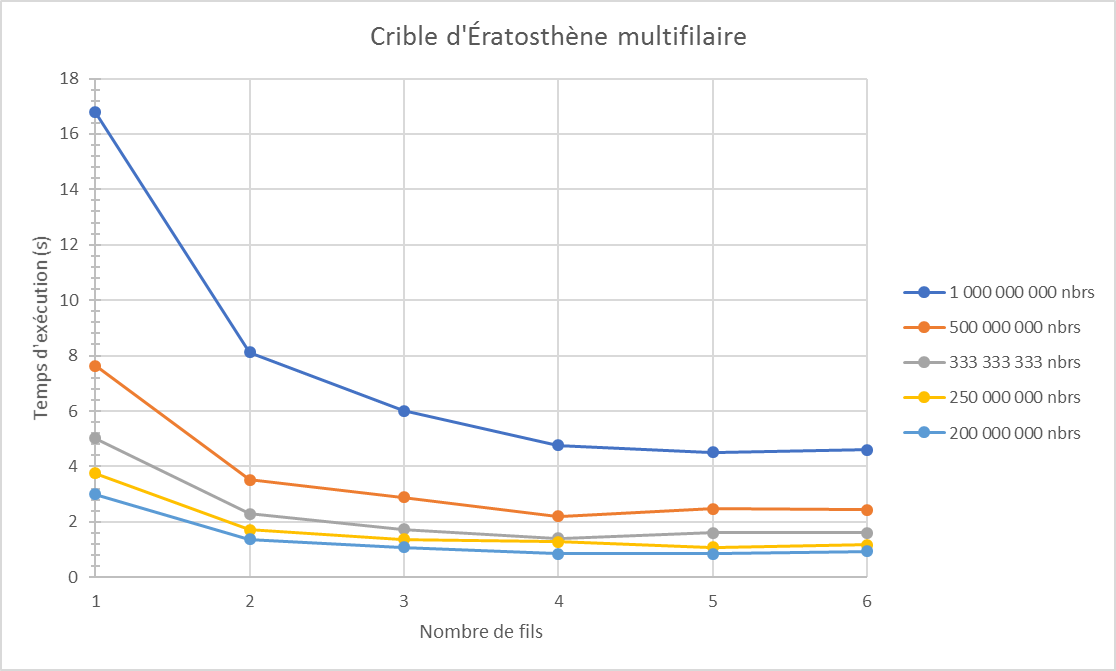
\includegraphics[scale=0.7]{Images/Graph_temps_exec.png}
		\caption{Comparaison des temps d'éxécution}
	\end{figure}
\end{center}

\begin{center}
	\begin{figure}[H]
		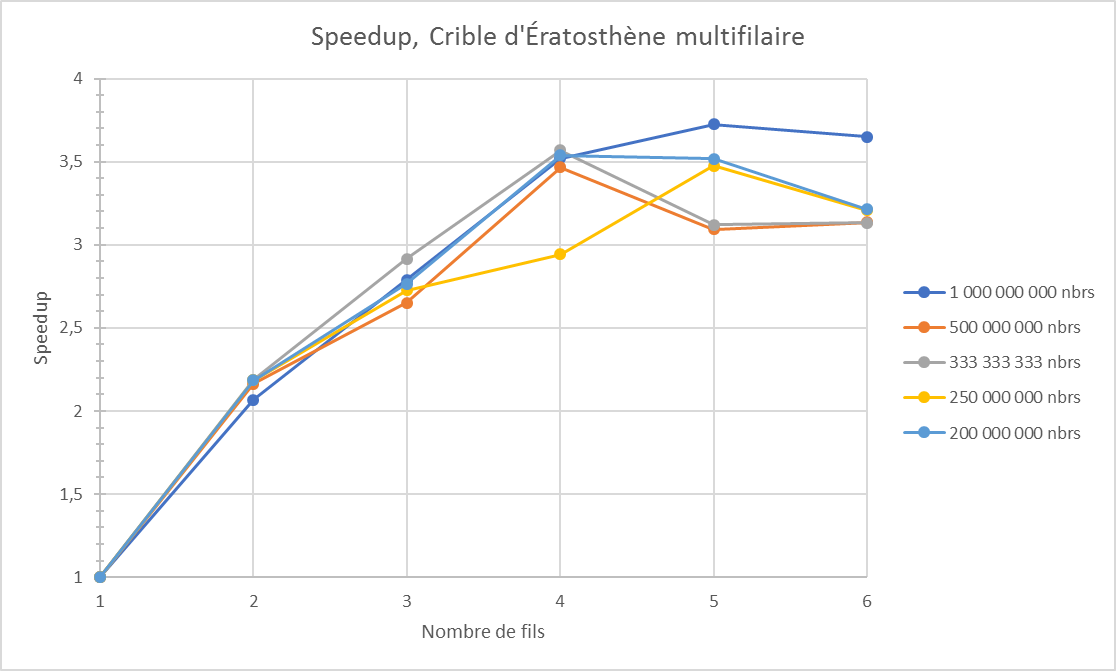
\includegraphics[scale=0.7]{Images/Graph_speedup.png}
		\caption{Comparaison du speedup selon le nombre de fil}
	\end{figure}
\end{center}

\begin{center}
	\begin{figure}[H]
		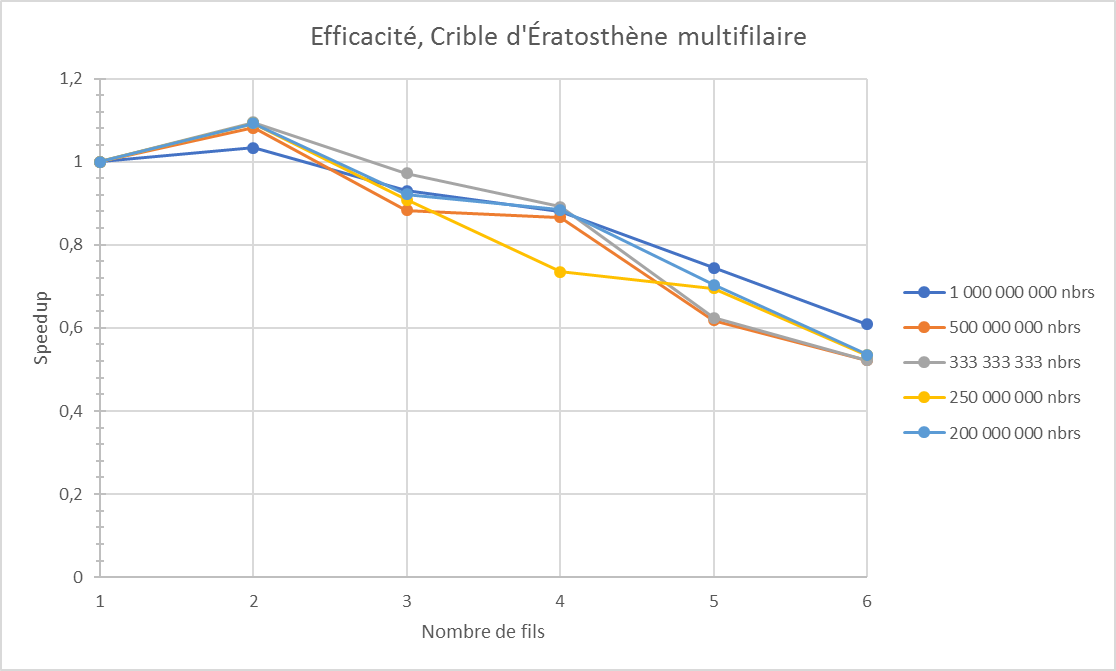
\includegraphics[scale=0.7]{Images/Graph_eff.png}
		\caption{Comparaison de l'éfficacité selon le nombre de fil}
	\end{figure}
\end{center}
\section{Interprétation}
	Comme le démontrent nos résultats, on peut voir un plafonnement rapide
	de l'amélioration apportée par la parallélisation de l'algorithme. Par
	exemple, pour 1 milliard de nombres, on voit qu'a $\sim 4.50$ secondes
	pour 5 fils, le programme plafonne et ralentit à 6 fils. Cela peut être
	dû au fait que les tests ont été réalisés sur un ordinateur dont le
	processeur n'a que 4 coeurs.

	\smallskip
	De plus, il est possible de voir que l'efficacité diminue selon le
	nombre de fils et que le speedup, lui, augmente de plus en plus lentement.
	Ce sont d'autres indicateurs du plafonnement de notre parallélisation.

	\bigskip
	Somme toute, notre meilleur résultat est obtenu lors de l'utilisation de 
	5 fils d'exécution pour 1 milliard de nombre, soit un speedup de $\sim 3.72$
	et une efficacité de $\sim 0.74$.

	\bigskip
	Il est possible, toutefois, d'appercevoir dans les graphiques et les tableaux
	précédents certaines anomalies: des valeurs de speedup plus grandes que le
	nombre de fils d'exécution utilisés, ainsi que des valeurs d'efficacité plus
	grandes que 1.

	\smallskip
	Nous somme d'avis que ces valeurs sont dûes à de petites variation dans la
	vitesse de traitement du processeur	pendant le test. L'erreur dans ces cas
	est de l'ordre de $\sim 9\%$ au maximum, dans les cas avec les plus petit
	nombre de valeurs à traiter.

	Pour 1 milliard de nombres, l'erreur se situe à $\sim 3\%$.

	\bigskip
	Nous avons tenté de rendre les fils d'exécution les plus indépendants
	possible les uns des autres. Pour ce faire, chaque fil fait le traitement
	du tableau en entier, en marquant les multiples d'un nombre donné en entrée.
	Dès que celui-ci a terminé, il prends le prochain nombre disponible afin de
	continuer le traitement sans interruption.

	\smallskip
	De plus, nous avons minimisé l'usage de mutex. Nous n'en utilisons qu'un seul
	dans le programme, au moment de modifier le prochain nombre à traiter. C'est le
	seul moment dans notre programme où il y aurait pu y avoir interférence entre
	une lecture et une écriture, donc nous avons appliqué un mutex. Pour marquer les
	nombre comme composés dans le tableau, nous incrémentons la valeur, donc même
	si dans le cas où 2 fils voudraient l'incrémenter en même temps, il n'y a pas
	de lecture à faire, donc pas de possibilité d'interférence.

\chapter{Conclusion}
Ce travail pratique nous a permis de faire des exéprimentaions afin de parralléliser l'algorithme du Crible d'Ératosthène.
Les résultats obtenus nous ont montré tous les bénéfice qu'on peut tirer de parralléliser un algorithme en terme de rapitdé
d'éxécution et d'éfficacité.
Cependant, Malgré nos résultats que nous considérons trés bons, nous n'avions pas les connaissances nécessaires ou le temps suffisant
pour apprendre les subtilités qui s'offrent à nous en terme d'utilisation des options d'optimisation du compilateur.
\end{document}

